\documentclass[twocolumn,linenumbers]{aastex631}
\usepackage{physics}
\usepackage{gensymb}
\usepackage{CJK}

% Operators
\DeclareMathOperator*{\argmax}{arg\,max}
\DeclareMathOperator*{\argmin}{arg\,min}
\DeclareMathOperator*{\diag}{diag}
\newcommand{\exptval}[1]{\mathbb{E}\left[ #1 \right]}
\newcommand{\Var}[1]{\text{Var}\qty[#1]}
\newcommand{\Cov}[1]{\text{Cov}\qty[#1]}

% variables
\newcommand{\bb}[1]{\mathbb{#1}}
\newcommand{\vbd}{\vb{d}}
\newcommand{\vbm}{\vb{m}}
\newcommand{\vbep}{\vb{\varepsilon}}
\newcommand{\vbn}{\vb{n}}
\newcommand{\vbb}{\vb{b}}
\newcommand{\inv}[1]{#1^{-1}}
\newcommand{\noisevar}{\Sigma_{\vbn}}
\newcommand{\hatm}{\vb{\hat{m}}}
\newcommand{\Pdagger}{P^{\dagger}}
\newcommand{\Nbar}{\bar{N}}
\newcommand{\PPinv}[1]{\inv{\qty(\Pdagger #1 P)}}
\newcommand{\Neta}{N_{\eta}}

\newcommand{\kmh}[1]{\textcolor{red}{KMH: #1}}


%\submitjournal{ApJ}
\graphicspath{{./}{figures/}}

\begin{document}

%\title{Perturbative Approach to Solve the Map-Making Equation}
%\title{Cosmic Microwave Background map-making solutions with a cooled or perturbative approach}
\title{Cosmic Microwave Background map-making solutions improve with cooling}


  \author{Bai-Qiang Qiang (\kmh{want chinese characters?})} % KMH: I don't know how to do it...
\affiliation{Department of Physics, Florida State University, Tallahassee, Florida 32306}

\author[0000-0001-7109-0099]{Kevin M. Huffenberger}
\affiliation{Department of Physics, Florida State University, Tallahassee, Florida 32306}

 
\begin{abstract}

In the context of Cosmic Microwave Background data analysis, we study the solution to the equation that transforms scanning data into a map.
As originally suggested in ``messenger'' methods for solving linear systems, we split the  noise covariance into uniform and non-uniform parts and adjusting their relative weight during the iterative solution.
This ``cooling'' or perturbative approach is particularly effective when there is significant low-frequency noise in the timestream.
A conjugate gradient algorithm applied to this modified system converges faster and to a higher fidelity solution than the standard conjugate gradient approach, for the same computational cost per iteration.
We conclude that ``cooling'' is helpful separate from its appearance in the messenger methods.
We give an analytical expression for the parameter that controls how gradually should change during the course of the solution. 

\end{abstract}

\keywords{Computational methods --- Cosmic microwave background radiation --- Astronomy data reduction}

\section{Introduction} \label{sec:intro}


In observations of the Cosmic Microwave Background (CMB), map-making is an intermediate step between the collection of raw scanning data and the scientific analyses, such as the estimation of power spectra and cosmological parameters.
Next generation CMB observations will generate much more data than those today, and so
it is worth exploring efficient ways to process the data, even though, on paper, the map-making problem has long been solved.

The time-ordered scanning data is summarized by
\begin{equation}
\vbd = P\vbm + \vbn \label{map making model}
\end{equation}
where $\vbd$, $\vbm$, and $\vbn$ are the vectors of time-ordered data (TOD), the CMB sky-map signal, and measurement noise.
$P$ is the sparse matrix that encodes the telescope's pointing.  Of several map-making methods \citep{1997ApJ...480L..87T}, one of the most common is the method introduced for the Cosmic Background Explorer \cite[COBE,][]{1992ASIC..359..391J}.  This optimal, linear solution is 
\begin{align}
\qty(\Pdagger \inv{N}  P) \hatm = \Pdagger \inv{N} \vbd \label{map making eq}
\end{align}
where  $\hatm$ provides the generalized least squares minimization of the $\chi^2$ statistic,

\begin{align}
\chi^2(\vbm) & \equiv (\vbd - P\vbm)^{\dagger} N^{-1} (\vbd - P \vbm).
\label{chi2 formula}
\end{align}
Here we assume that the noise has zero mean $\ev{\vbn} = \vb{0}$,
and noise covariance matrix $N = \ev{\vbn \vbn^{\dagger}}$ is diagonal in frequency space.
Thus  map-making is a standard linear regression problem.
In the case where the noise is Gaussian, the COBE solution is also the maximum likelihood solution.

With current computation power, we cannot solve for $\hatm$
by calculating $\PPinv{\inv{N}} \Pdagger \inv{N} \vbd$ directly.
The noise covariance matrix $N$ is often sparse in frequency domain and the pointing matrix $P$ is sparse in the time-by-pixel domain.
In experiments currently under design, there may be $\sim 10^{16}$ time samples and $\sim 10^{9}$ pixels, so these matrix inversions are intractable unless the covariance is uniform.
We can use iterative methods, such as conjugate gradient descent, to avoid the matrix inversions, and execute each matrix multiplication in a basis where the matrix is sparse, using a fast Fourier transform to go between the frequency and time domain.

As an alternative to conjugate gradient descent, \citet{Huffenberger_2018} showed that the ``messenger'' iterative method could be adapted to solve the linear map-making system, based on the  approach from \cite{2013A&A...549A.111E} to solve the linear Wiener filter.  This technique splits the noise covariance into a uniform part and the remainder, and introduces an additional vector that represent the signal plus uniform noise.  This messenger field acts as an intermediary between the signal and the data and has a covariance that is conveniently sparse in every basis.  \cite{2013A&A...549A.111E} also introduced a cooling scheme that takes  advantage of the split covariance: over the course of the iterative solution, we adjust the relative weight of the two parts.  Starting with the uniform covariance, the modified linear system gradually transforms to the final system, under the control of a cooling parameter.  In numerical experiments, \citet{Huffenberger_2018} found that a map produced by the cooled messenger method converged significantly faster than for standard conjugate gradient methods, and to higher fidelity, especially on large scales.  

\citet{2018A&A...620A..59P} showed that the the messenger field approach is equivalent to a fixed point iteration scheme, and studied its convergence properties in detail.  Furthermore, they showed that the split covariance and the modified system that incorporates the cooling can be solved by other means, including a conjugate gradient technique, which should generally show better convergence properties than the fixed-point scheme. However in numerical tests, \citet{2018A&A...620A..59P} did not find benefits to the cooling modification of the map-making system, in contrast to findings of \citet{Huffenberger_2018}.

In this paper, we show that the difference arose because the numerical tests in \citet{2018A&A...620A..59P} used much less low-frequency (or $1/f$) noise than \citet{Huffenberger_2018}, and show that the cooling technique improves map-making performance especially when the low-frequency noise is large.  This performance boost depends on a proper choice for the pace of cooling.  \citet{2017MNRAS.468.1782K} showed that for Wiener filter the cooling parameter should be chosen as a geometric series.  In this work, we give an alternative interpretation of the parameterizing process and show that for map-making the optimal choice (unsurprisingly) is also a geometric series.


In Section \ref{sec:methods} we describe our methods for treating the map-making equation and our numerical experiments.
In Section \ref{sec:results} we present our results. 
In Section \ref{sec:discussion} we intuitively interpret our method, and point out possible improvement direction.
Section \ref{sec:conclusions} is our conclusion.
In Appendix \ref{appendix:eta calculation} we derive the prescription for our ``cooling'' schedule.


\section{Methods}\label{sec:methods}

\subsection{Parameterized Conjugate Gradient Method}
The messenger field approach introduced an extra cooling parameter $\lambda$ to the
map-making equation, and solved the linear system with the alternative parameterized covariance $N(\lambda) =  \lambda \tau I + \Nbar $.
The parameter $\tau = \min(\diag(N))$ represents the uniform level of (white) noise in the original covariance.
$\Nbar \equiv N - \tau I$ is the non-uniform part of the original noise covariance.
(Notation alert $N$ without any arguments denotes the original noise covariance matrix $N = \ev{\vbn \vbn^{\dagger}}$.)
In this work we find it more convenient to work with the reciprocal of cooling parameter $\eta = \lambda^{-1}$
which represents the degree of heteroscedasticity in the parameterized covariance
\begin{equation}
  N(\eta) = \tau I +  \eta \Nbar 
\end{equation}
which leads to the same system of map-making equations.
(This is because $N(\eta) = \lambda^{-1} N(\lambda)$ and the map-making equation (\ref{map making eq eta}) is insensitive to to scalar multiple of the covariance since is appears on both sides.)
When $\eta=1$ this parameterized covariance $N(\eta)$ equals $N$.


\citet{2018A&A...620A..59P} showed that the conjugate gradient method can be easily applied to the cooled map-making problem.
In our notation, this is equivalent to iterating on the parameterized map-making equation
\begin{align}
  \qty(\Pdagger \inv{N(\eta_i)} P)\, \hatm(\eta_i) = \Pdagger \inv{N(\eta_i)} \vbd,
\label{map making eq eta}
\end{align}
as we adjust the parameter through a set of levels $\{\eta_i\}$.
Notation alert $\hatm$ without $\eta$ argument
means the estimated $\hatm$ in Eq.~(\ref{map making eq}),
independent of $\eta$.
In our numerical experiments, we confirm that the conjugate gradient approach is converging faster than the fixed point iterations suggested by the messenger map-making method in \citet{Huffenberger_2018}.  For simplicity we fix the preconditioner to $M= \Pdagger P$ for all of calculations.


When $\eta = 0$, the noise covariance matrix $N(0)$ is homoscedastic, and solution is given by simple binned map
$\hatm(0) = \inv{\qty(\Pdagger P)} \Pdagger \vbd$,
which can be solved directly.

Since the non-white part $\bar N$ is the troublesome portion of the covariance.
We can think of the $\eta$ parameter as increasing heteroscedasticity of the system,
adding a perturbation to the solution achieved at a particular stage,
building ultimately upon the initial uniform covariance model.
Therefore, this quasi-static process requires $\eta$ increase as $0 = \eta_0 \leq \eta_1 \leq \cdots \leq \eta_{\rm final} = 1$, at which point we arrive at the desired map-making equation,
and the solution $\hatm(1) = \hatm$.

We may iterate more than once at each intermediate $\eta_i$: we solve with conjugate gradient iterations
using the result from previous calculation $\hatm(\eta_{i-1})$ as the initial value,
and move to next parameter $\eta_{i+1}$ when the norm of residual vector 
\begin{align}
\norm{\vb{r}(\eta_i)} \equiv
\norm{ \Pdagger \inv{N(\eta_i)} P\, 
\hatm(\eta_i) - \Pdagger \inv{N(\eta_i)} \vbd  }
\end{align}
per pixel is smaller than a tenth of the pixel standard deviation given by the white noise level of the noise model.
\begin{align}
\frac{\norm{\vb{r}(\eta_i)} }{ \text{ total pixel number }}  < 0.1 {\sigma_{\rm pix}}
\label{norm threshold}
\end{align}



\subsection{Analytical expression for $\qty{\eta_i}$ series}
The next question is how to appropriately choose these monotonically increasing parameters
$\eta$. 
We also want to determine $\eta_1, \cdots, \eta_{n-1}$ before starting conjugate
gradient iterations,
because the time ordered data $\vbd$ is very large,
and we do not want to keep it in the system memory during calculation.
If we determine $\eta_1, \cdots, \eta_{n-1}$ before the iterations, 
then we can precompute the right-hand side of Eq.~(\ref{map making eq eta})
for each $\eta_i$ and keep these map-sized objects in memory, instead of the entire time-ordered data.

In the appendix \ref{appendix:eta calculation}, we show that a generic good choice for the $\eta$ parameters are the geometric series
\begin{align}
\eta_i =\min \qty\bigg{ \qty(2^i -1)\frac{\tau}{\max(\Nbar_f)},\; 1 },
\label{etai rule}
\end{align}
where $\bar N_f$ are the eigenvalues of $\Nbar$ under frequency representation.
This is our main result.
It tells us not only how to choose parameters $\eta_i$,
but also when we should stop the perturbation, and set $\eta = 1$.
For example, if noise covariance matrix $N$ is almost white noise,
then $\Nbar = N - \tau I \approx 0$,
and we would have ${\tau}/{\max(\Nbar_f)} > 1$.
This tell us that we don't need to use parameterized method at all, 
because $\eta_0=0$ and $\eta_1= \eta_2 = \cdots= 1$.
This corresponds to the standard conjugate gradient method with simple binned 
map as the initial guess (as recommended by \citealt{2018A&A...620A..59P}).


\subsection{Computational Cost}
To properly compare the performance cost of this method with respect to vanilla
conjugate gradient method with simple preconditioner,
we need to compare their computational cost at each iteration.
The right hand side of parameterized map-making equation
(\ref{map making eq eta})
could be computed before iterations,
since we have determined $\qty{\eta_i}$ in advance,
so it won't introduce extra computational cost.
The most demanding part of conjugate gradient method is calculating
its left hand side, because it contains a Fourier transform of
$P\vbm$ from time domain to frequency domain and an inverse Fourier transform
of $\inv{N(\eta_i)} P \vbm$ from frequency domain back to time domain,
which is order $\mathcal{O}(n\log n)$ with $n$ being the length of time ordered
data.
Compare to traditional conjugate gradient method,
we swap $\inv{N}$ with $\inv{N(\eta)}$, and it won't add extra cost,
since both methods need a fast Fourier transform and inverse fast Fourier transform 
at one iteration.
Therefore the computational cost it the same for one step.

In Appendix \ref{appendix:eta calculation}
our analysis is based on
$\chi^2(\hatm(\eta_i), \eta_i)$ which is evaluated at 
$\hatm(\eta_i)$ the estimated map at $\eta_i$.
So we should update $\eta_i$ to $\eta_{i+1}$ when the map from our calculation
$\vbm \approx \hatm(\eta_i)$. 
How do we know this condition is satisfied?
Since for each new $\eta_i$ value, we are solving a new set of linear
equations (\ref{map making eq eta}),
and we could stop calculation and moving to next value $\eta_{i+1}$ when the 
norm of residual $\norm{\vb{r}(\eta_i)}$ is small, see Eq.~(\ref{norm threshold}).
Calculate $\qty||\vb{r}(\eta_i)||$ is part of conjugate gradient algorithm,
so this won't add extra cost either.
Therefore, overall introducing $\eta$ won't have extra computational cost.



\subsection{Numerical Simulations}

\begin{figure}[tb!]
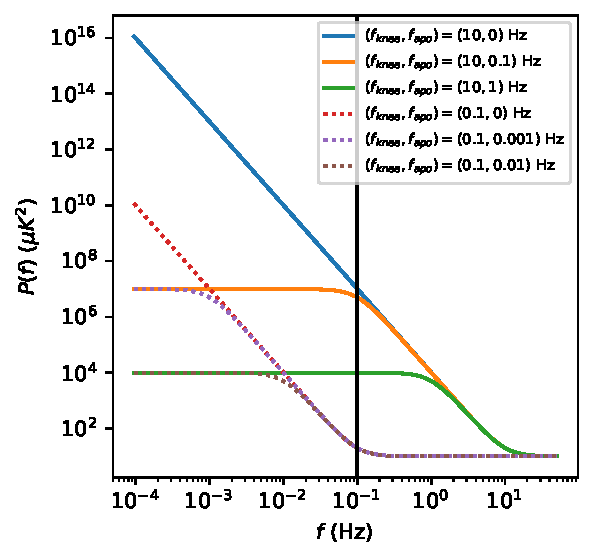
\includegraphics[width=\linewidth]{P_f.pdf}
\centering
\caption{The noise power spectrum based on Eq.~(\ref{noise power spectrum}) with 
    white noise level $\sigma^2 = 10$ $\mu$K$^2$ and low-frequency power-law slope $\alpha = 3$.
    Here shows two knee frequencies, $f_\text{knee}=10$ Hz (solid lines) 
    and $f_\text{knee}=0.1$ Hz (dashed lines).
    For each knee frequency, we have shown an unflattened spectrum ($f_\text{apo}=0$ Hz), and two flattened ones ($0.1f_\text{knee}$ and
    $0.01f_\text{knee}$).
    The vertical line shows our scanning frequency.
}
\label{power spectrum}
\end{figure}

To compare these algorithms, we need to do some simple simulation of scanning
processes, and generate time ordered data from a random sky signal.\footnote{
The source code and other information are available at \url{https://github.com/Bai-Qiang/map_making_perturbative_approach}
}
Our sky is a small rectangular area, with two orthogonal directions $x$ and
$y$, both with range from $-1\degree$ to $+1\degree$.
The signal has stokes parameters $(I,Q,U)$ for intensity and linear polarization.

For the scanning process, our mock telescope contains nine detectors,
each with different sensitivity to polarization $Q$ and $U$.
It scans the sky with a raster scanning pattern and scanning frequency
$f_{\text{scan}} = 0.1$ Hz and sampling frequency $f_{\text{sample}} = 100$ Hz.
The telescope scans the sky horizontally and then vertically,
and then digitizes the position $(x, y)$ into $512\times 512$ pixels.
This gives noiseless signal $\vb{s} = P\vb{m}$.

We model the noise power spectrum with
\begin{align}
P(f) = \sigma^2 \qty(1+ \frac{f_{\text{knee}}^{\alpha}+f_{\text{apo}}^{\alpha}}
    {f^{\alpha}+f_{\text{apo}}^{\alpha}}) \label{noise power spectrum}
\end{align}
which is white at high frequencies, a power law below the knee frequency, and gives us the option to flatten the low-frequency noise below an apodization frequency \citep[like in][]{2018A&A...620A..59P}.
Note that as $f_{\text{apo}} \rightarrow 0 $,
$P(f) \rightarrow \sigma^2\qty(1 + (f/f_{\text{knee}})^{-\alpha} )$, 
and it becomes a $1/f$ noise model.

\citet{2013ApJ...762...10D} measured the slopes of the atmospheric noise in the Atacama under different water vapor conditions, finding $\alpha = 2.7$ to $2.9$.
Here we fixed $\sigma^2 = 10$ $\mu$K$^2$, $\alpha=3$, and $f_{\text{knee}} = 10$ Hz,
and change $f_{\text{apo}}$ to compare the performance under different noise
models.

The noise covariance matrix 
\begin{equation}
N_{ff'} = P(f) \frac{\delta_{ff'}}{\Delta_f}
\label{noise covariance matrix}
\end{equation}
is a diagonal matrix in frequency space, where $\Delta_f$ is equal to reciprocal
of total scanning time $T \approx 1.05\times 10^{4}$ seconds.
In our calculations we choose different combination of $f_\text{knee}$ and $f_\text{apo}$,
some of the power spectrum are shown in Figure~\ref{power spectrum}.

Finally, we get the simulated time ordered data $\vb{d} = \vb{s} + \vb{n}$ by
adding up signal and noise.


\section{Results} \label{sec:results}

\begin{figure*}[tb!]
\centering
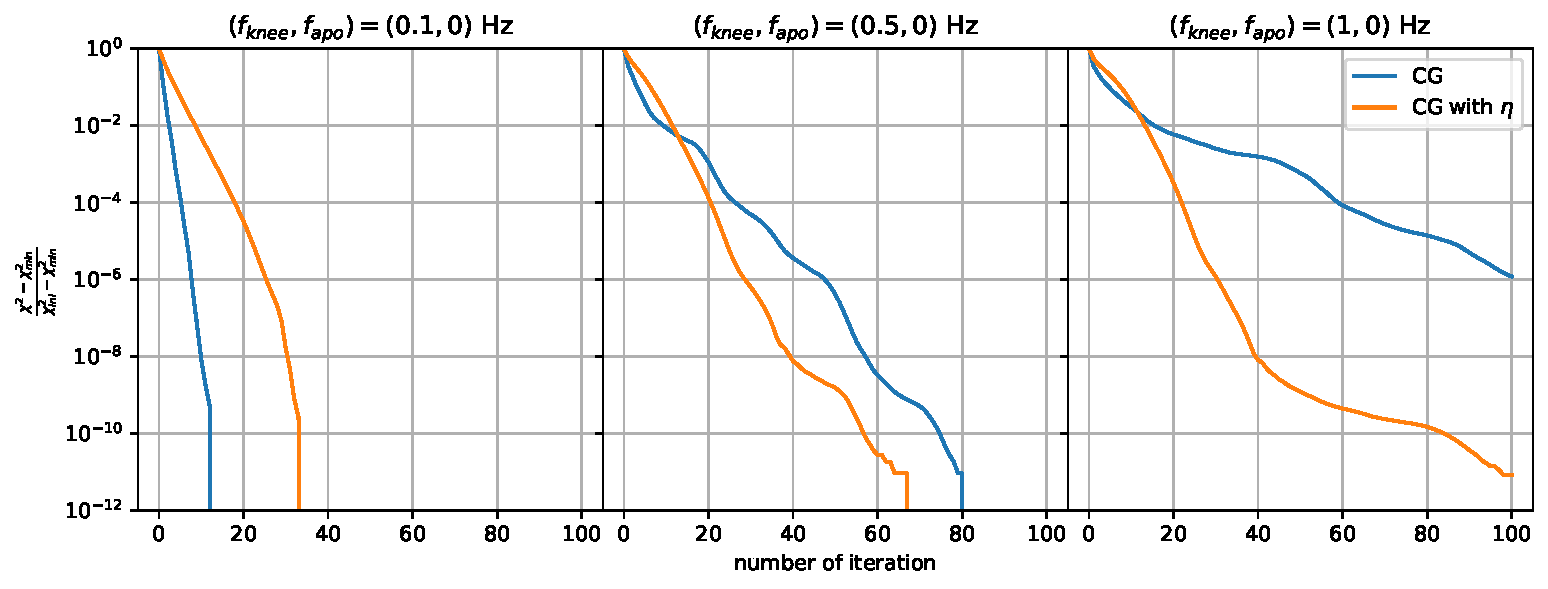
\includegraphics[width=0.8\textwidth]{pink_noise_chi2.pdf}
\caption{
    Here we show the $\chi^2(\vbm)$ with respect to number of iterations.
    The vertical axis is rescaled  such that all curves start from 1.
    The map-making equation (\ref{map making eq}) minimize the $\chi^2(\vbm)$, so
    the curve which goes down fast and get close to zero at the end is the preferred method.
    In this figure we are comparing traditional conjugate gradient method labeled as \textit{CG} (blue line)
    with parameterized conjugate gradient labeled as \textit{CG with $\eta$} (orange line)
    under different $1/f$ noise model (fixed $f_\text{apo}=0$ Hz but different $f_\text{knee}$ in Eq.(\ref{noise power spectrum})).
    As we can see here when $f_\text{knee} \gtrsim 10\,f_\text{scan} = 1$ Hz, there are significant amount of
    low-frequency noise and the parameterized conjugate gradient method starts showing advantages.
}
\label{1/f noise chi2}
\end{figure*}

\begin{figure*}[tb!]
\centering
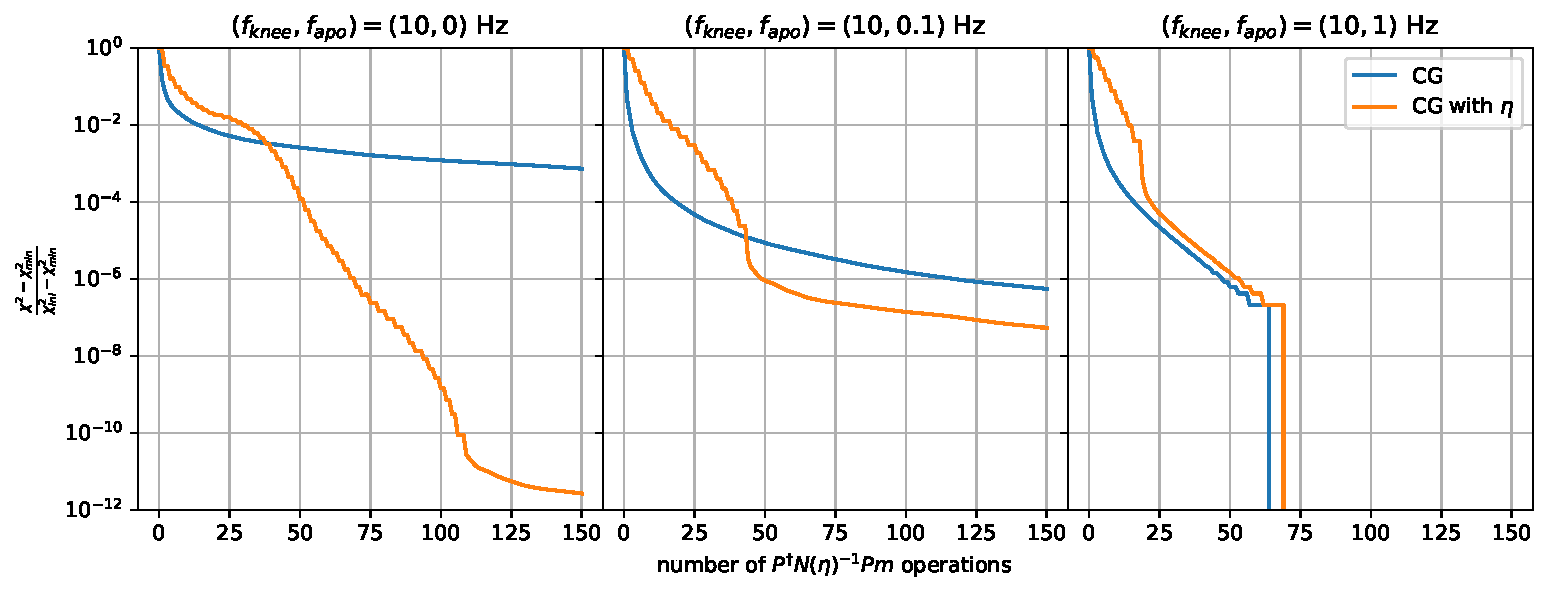
\includegraphics[width=0.8\textwidth]{flattened_noise_chi2.pdf}
\caption{
    The vertical and horizontal axes are the same as in Figure~\ref{1/f noise chi2},
    and also compare traditional conjugate gradient method labeled as \textit{CG} (blue line) 
    with parameterized conjugate gradient method labeled as \textit{CG with $\eta$} (orange line).
    But here we fix the knee frequency $f_\text{knee} = 10$ Hz, and change apodization frequency $f_\text{apo}$.
    When $f_\text{apo}$ is much smaller than $f_\text{knee}$, there are more low-frequency noise and
    parameterized conjugate gradient method is better than traditional ones.
}
\label{apo noise chi2}
\end{figure*}

We first compare the vanilla conjugate gradient method with
simple preconditioner $\Pdagger P$ versus conjugate gradient with our perturbed linear system.
Figure~\ref{1/f noise chi2} shows the $\chi^2(\vbm)$ results for 1/f noise model ($f_\text{apo}=0$)
with different knee frequencies.
Note that $\chi^2$ in all figures are calculated based on $\chi^2(\vbm)$ in Eq.~(\ref{chi2 formula})
not $\chi^2(\vbm, \eta)$ in Eq.~(\ref{chi2 eta formula}).
And the $\chi^2_{\text{min}}$ is calculated from parameterized conjugate gradient
method with 100 $\eta$ values, and it stops when the final norm of residual $\norm{\vb{r}(1)}$
per pixel is smaller than $10^{-10}\mu$K, or after 1000 iterations.
From Figure~\ref{1/f noise chi2} we can see for $1/f$ noise model,
when $f_\text{knee} \gtrsim 10 f_\text{scan}$ the parameterized method starts showing advantage
over vanilla conjugate gradient method.


In Figure~\ref{apo noise chi2} we fixed $f_\text{knee}=10$ Hz, and change $f_\text{apo}$.
When $f_\text{apo}$ is much smaller than $f_\text{knee}$ the parameterized conjugate gradient method would
performs better.
As we increase $f_\text{apo}$ while fix $f_\text{knee}$, eventually these two methods perform similar.

If we look at the power spectrum in Figure~\ref{power spectrum},
when $f_\text{knee}$ is small or $f_\text{apo}$ is large there are not many
large scale low-frequency noise.
So we conclude that by introducing $\eta$ parameter could improve perform when there are large low noise
contribution.


We also tried different $\alpha$ values. For $\alpha=2$, the conclusion is the
same as $\alpha=3$. When $\alpha=1$, there are not many low-frequency noise, 
the vanilla conjugate gradient is preferred, except some cases with very large
knee frequency like $f_\text{knee} = 100$ Hz and $f_\text{apo}=0$ would favor
parameterized method.
In \citealt{2018A&A...620A..59P}, the $\alpha = 1$ and  the noise power spectrum is flattened at $0.1f_\text{knee}$,
which corresponds to $f_\text{apo} \approx 0.1 f_\text{knee}$,
and their knee frequency is the same as scanning frequency, so $f_\text{knee}=f_\text{scan}=0.1$ 
in our cases.
In their case there are not many low-frequency noise,
and we confirm that vanilla conjugate gradient method would converge faster.



\section{Discussion} \label{sec:discussion}

\subsection{Intuitive Interpretation of $\eta$}\label{intuitive interp}


Here is another way to interpret the role of $\eta$ in addition to Appendix \ref{appendix:eta calculation}.
Our ultimate goal is to find $\hatm(1)$ which minimizes $\chi^2(\vbm)$ in Eq.~(\ref{chi2 formula}).
Since $N$ is diagonal in frequency space,
$\chi^2$ could be written as a sum of all frequency mode
$\qty|(\vbd-P\vbm)_f|^2$ with weight $\inv{N}_f$, such as
$\chi^2(\vbm) = \sum_f \qty|(\vbd-P\vbm)_f|^2 \inv{N}_f$.
The weight is large for low noise frequency mode (small $N_f$), and vice versa.
Which means $\chi^2(\vbm)$ would favor the low noise frequency mode over high
noise ones.
In other words the optimal map $\hatm$ focusing on minimize the error
$\vb*{\varepsilon} \equiv \vbd - P\vbm$ in the low-noise part.

After introducing $\eta$, we minimize
$\chi^2(\vbm,\eta)$ in Eq.~(\ref{chi2 eta formula}) instead.
For $\eta=0$, $N^{-1}(0) \propto I$ the system is homoscedastic and the estimated map $\hatm(0)$
does not prioritize any frequency mode.
As we slowly increase $\eta$, we decrease the weight for the high noise modes,
and focusing minimizing error for low noise part.
If we start with $\eta_1=1$ directly, which corresponds to the vanilla conjugate
gradient method, then the entire conjugate gradient solver
will focus most on minimizing the low noise part, such that $\chi^2$ would
converge very fast at low noise region, but slowly on high noise part.
It may be stuck at some local minimum point and hard to get to global minimum.
However by introducing $\eta$ parameter, we let the solver first treat every
frequency equally,
then as $\eta$ slowly increases, it gradually give more focus to the lowest noise part.



\subsection{Other $\eta$ Choices}

\begin{figure*}[tb!]
\centering
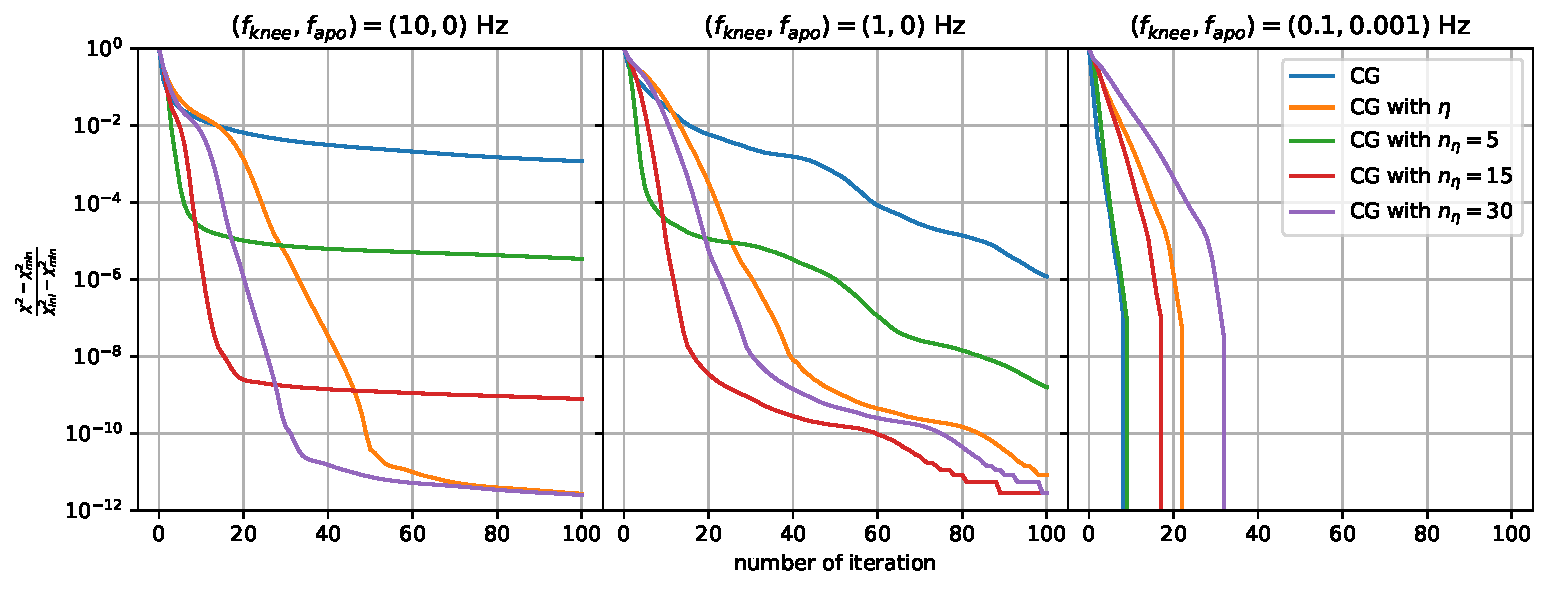
\includegraphics[width=0.8\textwidth]{chi2_neta.pdf}
\caption{
    The horizontal and vertical axes are the same as in the previous figure.
    The blue line and the orange line are traditional conjugate gradient method
    and parameterized conjugate gradient method.
    For three extra lines, we fix the number of $\eta$ parameter $n_{\eta}$ manually.
    The $\eta$ series are determined by Eq.~(\ref{neta eq}).
    The first graph shows in some cases the $\eta$ series given by Eq.~(\ref{etai rule}) is ideal,
    but the second and third graph show that Eq.~(\ref{etai rule}) may ends up too many $\eta$
    which yields slower convergence.
}
\label{chi2 neta}
\end{figure*}

Now let us compare the performance difference between choosing $\eta$
parameters based on Eq.~(\ref{etai rule})
and fixing number of $\eta$ parameters $n_{\eta}$ manually then
choose the $\eta_i$ from this geometric series
\begin{align}
\eta_i = \eta_1^{\frac{n_{\eta}-i}{n_{\eta} - 1}} \ \textrm{ with } i=1,2,\cdots,n_{\eta}
\label{neta eq}
\end{align}
with $\eta_1 = \tau/\max(\Nbar_f)$.

The results are showed in Figure~\ref{chi2 neta}.
In some cases the $\eta$ series determined by Eq.~(\ref{etai rule}) is ideal
(the first graph in Figure~\ref{chi2 neta}), in other cases Eq.~(\ref{etai rule})
gives too many $\eta$ values such that it is not optimal (the second and third
graph in Figure~\ref{chi2 neta}).
So we need to find a way to improve Eq.(\ref{etai rule}).



\subsection{Future Prospects}

\begin{figure*}[tb!]
\centering
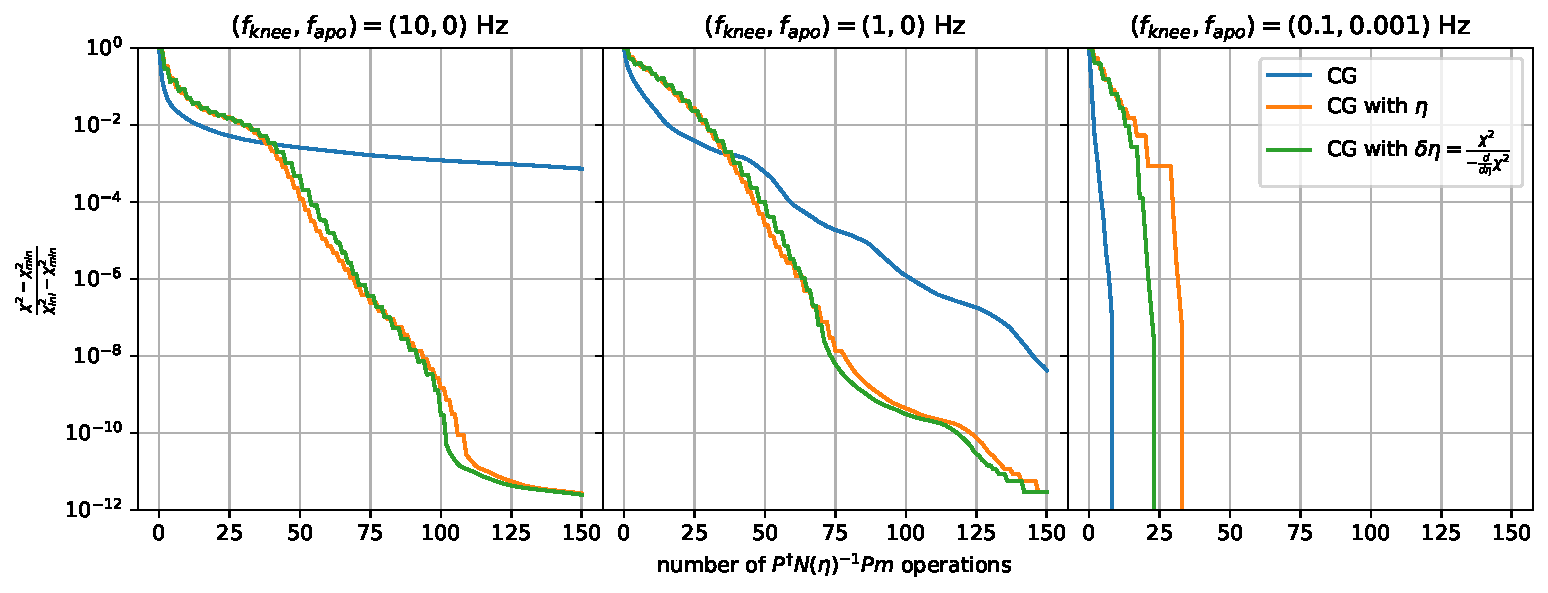
\includegraphics[width=0.8\textwidth]{chi2_exact_eta.pdf}
\caption{
    The blue line and orange line is the same as in Figure~\ref{chi2 neta} for reference.
    The extra green line shows the result when $\delta\eta_m$ is determined from 
    Eq.~(\ref{exact eta}) not from Eq.~(\ref{etai rule}).
    This shows that if we could update based on exact expression Eq.~(\ref{exact eta}),
    it could converge even faster.
    Especially in the third graph it would overcome the shortcomings of parameterized conjugate gradient method.
}
\label{chi2 exact eta}
\end{figure*}

In Appendix~\ref{appendix:eta calculation}, we determine $\delta\eta_m$ value based on the least upper bound of 
$-\delta\chi^2(\hatm(\eta_m), \eta_m)/\chi^2(\hatm(\eta_m), \eta_m)$, and choose $\delta\eta_m$ such that 
the least upper bound is equal to $1$.
The reason we use this upper bound instead of using
\begin{align}
\delta\eta_m=-\chi^2(\hatm(\eta_m), \eta_m)/\dv{\eta}\chi^2(\hatm(\eta_m),\eta_m)
\label{exact eta}
\end{align}
directly, is that we don't want to keep the time ordered data $\vbd$ in system memory.
But we could do this in simulations.
In Figure~\ref{chi2 exact eta} we can see if we use Eq.~(\ref{exact eta}), indeed it can improve performance. 
Especially for the third graph where the power spectrum does not have lots of
low-frequency noise.
This performance could get close to vanilla conjugate gradient method
when there is no significant amount of low-frequency noise,
which overcomes the shortcomings of parameterized conjugate gradient method.
Therefore, to further improve this method, we need to find more accurate expression for Eq.~(\ref{dchi2 chi2})
and Eq.~(\ref{exact eta}).



\section{Conclusions} \label{sec:conclusions} 


We presented a parameterized conjugate gradient method with parameter $\eta$ based on the idea of messenger field
separating the white noise out of noise covariance matrix.
Then we gave an analytical expression for $\eta$ series,
and showed that this method would not introduce extra computational cost than traditional conjugate method.

We tested this method under different power spectrum both flattened and non-flattened.
The results showed that this method is faster than traditional conjugate gradient method 
when there are significant amount of low-frequency noise.
But it could be further improved if we could get more accurate estimation for Eq.~(\ref{exact eta}),
either before iteration or without using time ordered data during iteration.

Also note that we fixed preconditioner as $M = \Pdagger P$ during our calculation,
this parameterizing process could be applied to any preconditioner and possibly improve performance when 
there are significant amount of low-frequency noise.

\citet{2018A&A...620A..59P} showed that the messenger field method solving Wiener
filter problem introduced by \cite{2013A&A...549A.111E} could also be written as 
parameterized conjugate gradient algorithm.
Then \citet{2017MNRAS.468.1782K} introduced dual messenger field method to Wiener filter.
If applying our idea to Wiener filter problem, hopefully, it may also bring improvements.













%% IMPORTANT! The old "\acknowledgment" command has be depreciated. It was
%% not robust enough to handle our new dual anonymous review requirements and
%% thus been replaced with the acknowledgment environment. If you try to 
%% compile with \acknowledgment you will get an error print to the screen
%% and in the compiled pdf.
\begin{acknowledgments}
BQ and KH are supported by NSF award 1815887.
\end{acknowledgments}

%% To help institutions obtain information on the effectiveness of their 
%% telescopes the AAS Journals has created a group of keywords for telescope 
%% facilities.
%
%% Following the acknowledgments section, use the following syntax and the
%% \facility{} or \facilities{} macros to list the keywords of facilities used 
%% in the research for the paper.  Each keyword is check against the master 
%% list during copy editing.  Individual instruments can be provided in 
%% parentheses, after the keyword, but they are not verified.

%\vspace{5mm}
%\facilities{HST(STIS), Swift(XRT and UVOT), AAVSO, CTIO:1.3m,
%CTIO:1.5m,CXO}

%% Similar to \facility{}, there is the optional \software command to allow 
%% authors a place to specify which programs were used during the creation of 
%% the manuscript. Authors should list each code and include either a
%% citation or url to the code inside ()s when available.

%\software{astropy \citep{2013A&A...558A..33A,2018AJ....156..123A},  
%          Cloudy \citep{2013RMxAA..49..137F}, 
%          Source Extractor \citep{1996A&AS..117..393B}
%          }

%% Appendix material should be preceded with a single \appendix command.
%% There should be a \section command for each appendix. Mark appendix
%% subsections with the same markup you use in the main body of the paper.

%% Each Appendix (indicated with \section) will be lettered A, B, C, etc.
%% The equation counter will reset when it encounters the \appendix
%% command and will number appendix equations (A1), (A2), etc. The
%% Figure and Table counter will not reset.


%%%%%%%%%%%%%%%%%%%%%%%%%%%%%%%%%%%%%%%%%%%%%%%%%%%%%%%%%%%%%%%%%%%
%%%%%%%%%%%%%%%%%%%%%%%%%%%%%%%%%%%%%%%%%%%%%%%%%%%%%%%%%%%%%%%%%%%%
%
% APPENDIX
%
%%%%%%%%%%%%%%%%%%%%%%%%%%%%%%%%%%%%%%%%%%%%%%%%%%%%%%%%%%%%%%%%%%%%%%
%%%%%%%%%%%%%%%%%%%%%%%%%%%%%%%%%%%%%%%%%%%%%%%%%%%%%%%%%%%%%%%%%%%%%%%
\appendix
\section{The derivation of $\eta$ series} \label{appendix:eta calculation}

We know that initial degree of heteroscedasticity $\eta_0 = 0$,
which means the system is homoscedastic.
What would be good value for the next parameter $\eta_1$?
To simplify notation, we use $\Neta$ to denote the parameterized covariance $N(\eta) = \tau I +  \eta \bar N$.
For some specific $\eta$ value, the estimated map $\hatm(\eta) = \PPinv{\inv{\Neta}} \Pdagger \inv{\Neta} \vbd$ minimizes
\begin{align}
\begin{aligned}[b]
\chi^2 (\vbm, \eta)
&= \qty\big(\vbd - P \vbm)^{\dagger} \inv{\Neta} 
    \qty\big(\vbd - P\vbm).
\label{chi2 eta formula}
\end{aligned}
\end{align}
with $\eta$ being fixed.
We restrict to the case that the noise covariance matrix
$N$ is diagonal in the frequency domain, and represent the frequency-domain eigenvalues as $N_f$.

Let us first consider $\eta_1 = \eta_0 + \delta\eta = \delta\eta$
such that $\eta_1 = \delta \eta$ is very small quantity, $\delta \eta \ll 1$.
Since $\hatm(\eta)$ minimizes $\chi^2(\vbm,\eta)$ with $\eta$ being fixed, we have 
$\pdv{\hatm} \chi^2(\hatm(\eta), \eta) = 0$,
and using the chain rule
\begin{align}
\dv{\eta} \chi^2(\hatm(\eta), \eta) = \pdv{\eta} \chi^2(\hatm(\eta), \eta) 
= - \qty(\vbd - P\hatm(\eta))^{\dagger} \inv{\Neta} \Nbar \inv{\Neta}
    (\vbd - P\hatm(\eta)) \label{d chi2}
\end{align}
Then the fractional decrease of $\chi^2(\hatm(0),0)$ from $\eta_0= 0$ to 
$\eta_1 = \delta \eta$ is
\begin{align}
-\frac{\delta \chi^2(\hatm(0), 0)}{\chi^2(\hatm(0), 0)} 
= - \delta \eta \frac{\dv{\eta} \chi^2(\hatm(0),0)}{\chi^2(\hatm(0),0)}
&= \delta \eta 
\frac{1}{\tau}
\frac{\qty(\vbd - P\hatm(0))^{\dagger} \Nbar  (\vbd - P\hatm(0)) }
    {\qty\big(\vbd - P \hatm(0))^{\dagger} \qty\big(\vbd - P\hatm(0))}
\label{chi2 fractional decrease}
\end{align}
Here we put a minus sign in front of this expression such that it's 
non-negative, and use $N_{\eta=0} = \tau I$ at the second equality.
We want $\qty|\delta \chi^2(\hatm(0),0)| = \chi^2(\hatm(0),0)) - \chi^2(\hatm(\eta_1), \eta_1)$
to be large such that it could converge fast.
Let's say $\chi^2(\hatm(\eta_1), \eta_1)$ is much smaller than $\chi^2(\hatm(0), 0)$,
or $\chi^2(\hatm(\eta_1), \eta_1) \ll \chi^2(\hatm(0), 0)$.
Then we would expect
\begin{align}
-\frac{\delta\chi^2(\hatm(0),0)}{\chi^2(\hatm(0),0)}
= 1 - \frac{\chi^2(\hatm(\eta_1),\eta_1)}{\chi^2(\hatm(0),0)}
\approx 1^-
\label{dchi2/chi2 0}
\end{align}
The upper bound is strictly smaller than 1.
Now we could use Eq.(\ref{chi2 fractional decrease}) and let it equal to $1$, then
$\delta\eta=-\chi^2(\hatm(0), 0)/\dv{\eta}\chi^2(\hatm(0),0)$.
If we use this idea for $\eta_{m+1} = \eta_m + \delta \eta_m$ with $m \geq 1$, we would get
$ \delta\eta_m = -\chi^2(\hatm(\eta_m), \eta_m)/\dv{\eta}\chi^2(\hatm(\eta_m),\eta_m) $.
But as mentioned before, we need to determine the entire series $\qty{\eta_i}$ before conjugate gradient iterations,
and we could not calculate $\hatm(\eta_m)$ directly because of the difficulty of matrix inversions.
Therefore we could not get $\delta \eta_m$ values in advance.
That means we need to find another approach.

Let us go back to Eq.(\ref{chi2 fractional decrease}).
Since it is hard to analyze $\vbd - P\hatm(\eta)$ under frequency domain,
we treat it as an arbitrary vector, then the least upper bound is given by
\begin{align}
-\frac{\delta \chi^2(\hatm(0), 0)}{\chi^2(\hatm(0), 0)} 
\leq \frac{\delta \eta} {\tau} \max(\Nbar_f)
\label{dchi2/chi2 upper bound}
\end{align}
where $\max(\Nbar_f)$ is the maximum eigenvalue of $\Nbar$.
Now let us combine Eq.~(\ref{dchi2/chi2 0}) and Eq.~(\ref{dchi2/chi2 upper bound}).
We can choose $\delta \eta$ such that the least upper bound is equal to 1.
Thus we have
\begin{equation}
\eta_1 = \frac{\tau}{\max(\Nbar_f)} = \frac{\min(N_f)}{\max(N_f) - \min(N_f)}.
\end{equation}
Here $N_f$ and $\Nbar_f$ are the eigenvalues of $N$ and $\Nbar$ in the frequency
domain.
If the condition number of noise covariance matrix
$\kappa(N) = \max(N_f)/\min(N_f) \gg 1$,
then $\eta_1 \approx \inv{\kappa} (N)$.

What about the other parameters $\eta_m$ with $m > 1$?
We use a similar analysis,
letting $\eta_{m+1} = \eta_m + \delta \eta_m$ with a small $\delta\eta_m \ll 1$.
First, let us find the least upper bound
\begin{align}
-\frac{\delta \chi^2(\hatm(\eta_m), \eta_m)}{\chi^2(\hatm(\eta_m), \eta_m)}  
=& \delta\eta_m
\frac{\qty(\vbd - P\hatm(\eta_m))^{\dagger}
    \inv{N_{\eta_m}} \Nbar \inv{N_{\eta_m}}
    (\vbd - P\hatm(\eta_m))
}
{\qty\big(\vbd - P \hatm(\eta_m))^{\dagger}
    \inv{N_{\eta_m}}
    \qty\big(\vbd - P\hatm(\eta_m))
}
\label{dchi2 chi2}
\\
\leq & \delta \eta_m\, \max\qty(\frac{\Nbar_f}{\tau + \eta_m \Nbar_f})
\end{align}
The upper bound in the second line is a little bit tricky.
Both matrix $\Nbar$ and $\inv{N}_{\eta_m}$ 
can be simultaneously diagonalized in frequency space.
For each eigenvector $\vb{e}_f$,
the corresponding eigenvalue of the matrix on the numerator
$\inv{N}_{\eta_m} \Nbar \inv{N}_{\eta_m}$
is
$\lambda_f = \Nbar_f (\tau + \eta_m \Nbar_f)^{-2}$,
and the eigenvalue for matrix on the denominator
$\inv{N}_{\eta_m}$
is
$\gamma_f = (\tau + \eta_m \Nbar_f)^{-1}$.
Their eigenvalues are related by
$\lambda_f = [{\Nbar_f}/{(\tau + \eta_m \Nbar_f)}] \gamma_f$.
For any vector $\vb{v} = \sum_f \alpha_f \vb{e}_f$, we have
\begin{equation}
  \frac{\vb{v}^{\dagger} \inv{N}_{\eta_m} \Nbar \inv{N}_{\eta_m} \vb{v}}
{\vb{v}^{\dagger} \inv{N}_{\eta_m} \vb{v}}
= \frac{\sum_f \alpha_f^2 \lambda_f}{\sum_f \alpha_f^2 \gamma_f}
= \frac{\sum_f \alpha_f^2 \gamma_f \Nbar_f/(\tau + \eta_m \Nbar_f)}
{\sum_f \alpha_f^2 \gamma_f}
\leq \max \qty( \frac{\Nbar_f}{\tau + \eta_m \Nbar_f}).
\end{equation}

Again assuming $\chi^2(\hatm(\eta_{m+1}), \eta_{m+1}) \ll \chi^2(\hatm(\eta_m), \eta_m)$,
which we expect it to be satisfied for $ \eta_m \ll 1$.
That is because if $\eta \lesssim 1$, $\chi^2(\hatm(\eta), \eta)$ would close to the minimum $\chi^2$
which means $\chi^2(\hatm(\eta_{m+1}), \eta_{m+1}) \lesssim \chi^2(\hatm(\eta_m), \eta_m)$,
which would violate our assumption.
Luckily, the final result (\ref{etai rule appendix}) is a geometric series,
only the last few $\eta_m$ values fail to satisfy this condition.
Similarly, we could set the least upper bound equal to 1.
Then we get
\begin{align}
\delta \eta_m 
= \min \qty(\frac{\tau + \eta_m \Nbar_f}{\Nbar_f})
= \eta_m + \frac{\tau }{\max(\Nbar_f)}.
\end{align}
Therefore 
\begin{align}
\eta_{m+1} = \eta_m + \delta\eta_m = 2\eta_m + \frac{\tau }{\max (\Nbar_f)}
\end{align}
The final term ${\tau }/{\max (\Nbar_f)} = \eta_1$ becomes subdominant after a few terms, and we see that the $\eta_m$ increase like a geometric series. 
If written in the form $\eta_{m+1} + {\tau }/{\max(\Nbar_f)}
= 2 \qty( \eta_m + {\tau}/{\max(\Nbar_f)})$
it's easy to see that for $m \geq 1$,
$\eta_{m} + {\tau }/{\max(\Nbar_f)}$ forms a geometric series
\begin{align}
\eta_m +  \frac{\tau }{\max(\Nbar_f)}
=\qty(\eta_1 + \frac{\tau }{\max(\Nbar_f)}) 2^{m-1}
=\frac{\tau}{\max(\Nbar_f)} 2^m
\end{align}
where we used $\eta_1 = {\tau}/{\max(\bar{N}_f)}$.
Note that $m = 0$ and $\eta_0 = 0$ also satisfy this expression and we've got
final expression for all $\eta_m$
\begin{align}
\eta_m =\min \qty\bigg{1,\; \frac{\tau}{\max(\Nbar_f)} \qty(2^m -1) }
\label{etai rule appendix}
\end{align}
Here we need to truncate the series when $\eta_m > 1$.




 






%% For this sample we use BibTeX plus aasjournals.bst to generate the
%% the bibliography. The sample631.bib file was populated from ADS. To
%% get the citations to show in the compiled file do the following:
%%
%% pdflatex sample631.tex
%% bibtext sample631
%% pdflatex sample631.tex
%% pdflatex sample631.tex

\bibliography{references.bib}{}
\bibliographystyle{aasjournal}

%% This command is needed to show the entire author+affiliation list when
%% the collaboration and author truncation commands are used.  It has to
%% go at the end of the manuscript.
%\allauthors

%% Include this line if you are using the \added, \replaced, \deleted
%% commands to see a summary list of all changes at the end of the article.
%\listofchanges

\end{document}

% End of file `sample631.tex'.
